\section{Amplificatore alle differenze}
\begin{wrapfigure}[20]{r}[0pt]{55mm}
	\caption{Schema dell'amplificatore alle differenze}
	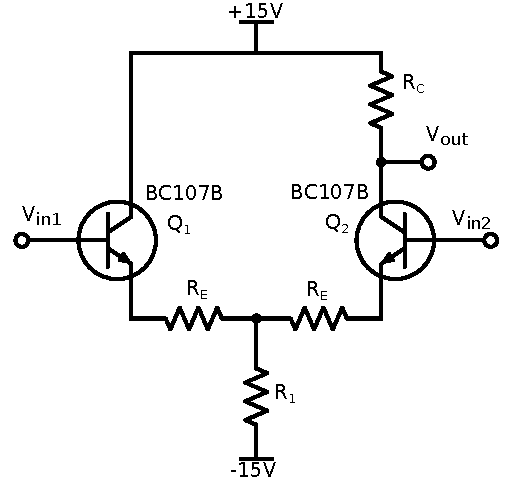
\includegraphics[width=55mm]{cc1.pdf}
	\label{fig:cc1}
\end{wrapfigure}

Un amplificatore alle differenze è un circuito che amplifica la differenza di due segnali in ingresso.
Il nostro obiettivo è quello di ottenere un circuito con una corrente di quiescenza $I_q=\SI{0.5}{\milli\ampere}$, un guadagno differenziale $G_{diff}\approx 30$ e un guadagno a modo comune $G_{CM} \leq 1$.
Il circuito da noi realizzato è rappresentato in Fig. \ref{fig:cc1}.

Per ottenere tali valori di corrente e guadagno sarebbe stato necessario dimensionare le resistenze del circuito, ma per questioni di tempo abbiamo scelto di utilizzare i valori delle resistenze fornitici dagli assistenti di laboratorio.

Abbiamo comunque cercato di stimare i valori di $R_1$ ed $R_E$ partendo da formule teoriche.
Una prima condizione è imposta da:

\begin{equation}
\SI{15}{\volt} \,= \, 2I_q R_1 + I_q R_E + \SI{0.6}{\volt}
\label{eq:1}
\end{equation}

\noindent Tale equazione tiene conto della geometria del circuito, tuttavia non permette da sola il calcolo di $R_E$ ed $R_1$.
Per fare ciò è necessario imporre una seconda condizione. Sia $r_e$ resistenza intrinseca dell'emettitore, vale:

\begin{equation}
G_{diff}=\frac{R_C}{2(R_E+r_e)} = 30
\label{eq:2}
\end{equation}

La resistenza intrinseca di emettitore $r_e$, come abbiamo appreso dallo studio del modello di \textit{Ebers-Moll}, può essere stimata dall'equazione sperimentale $r_e = \left[ \frac{25}{I_q} \right] \Omega$.
Imponendo pertanto una corrente di quiescenza di $I_q = \SI{0.5}{\milli\ampere}$ otteniamo immediatamente $r_e = 50\, \Omega$.

Infine, decidendo arbitrariamente il valore della resistenza $R_C=(9.972\pm0.002),\si{\kilo\ohm}$, è possibile stimare i valori adeguati di $R_1$ ed $R_E$, attraverso eq. (\ref{eq:1}) ed eq. (\ref{eq:2}). 
I valori di $R_E$ ed $R_1$ ricavati da eq. (\ref{eq:1}) ed eq. (\ref{eq:2}) sono:

$$R_E \, = \, \SI{116.667}{\ohm} \qquad \qquad \qquad R_1 \, = \, \SI{14.342}{\kilo\ohm}$$

\noindent Inoltre, la condizione sul guadagno a modo comune impone:

\begin{equation}
	\left| G_{CM} \right| \, = \, \left|  - \frac{R_C}{2 R_1 + R_E + r_e} \right| \, \leq \, 1
	\label{eq:3}
\end{equation}

da cui si ottiene:

$$	R_1 \, \geq \, \frac{1}{2} \left( R_C - R_E - r_e \right) \, = \, \SI{4.917}{\kilo\ohm}	$$

\noindent Il valore di $R_1$ viene pertanto verificato anche da eq. (\ref{eq:3})

Come consigliato in laboratorio, sono state utilizzate una $R_E=(118.9\pm0.5) \,\Omega$\footnote{In questo caso abbiamo scelto di eseguire un valor medio dei due valori misurati con il multimetro e di stimare un errore massimo definito come la semi-differenza dei due valori. Così facendo anche invertendo le resistenze nel circuito il valore reale sarà sempre compatibile con quello assunto nei calcoli.} e una $R_1= (9.933 \pm 0.002)\,\si{\kilo\ohm}$.
Con questi valori di resistenza la corrente di quiescenza $I_q$ è di \SI{0.7}{\milli\ampere} (sperimentalmente abbiamo misurato una corrente di $(0.719 \pm 0.003) \si{\milli\ampere}$.

Riportiamo ora (in Fig. \ref{fig:sig}) un grafico dei dati sperimentali acquisiti. 

\begin{figure}[h]
\centering
	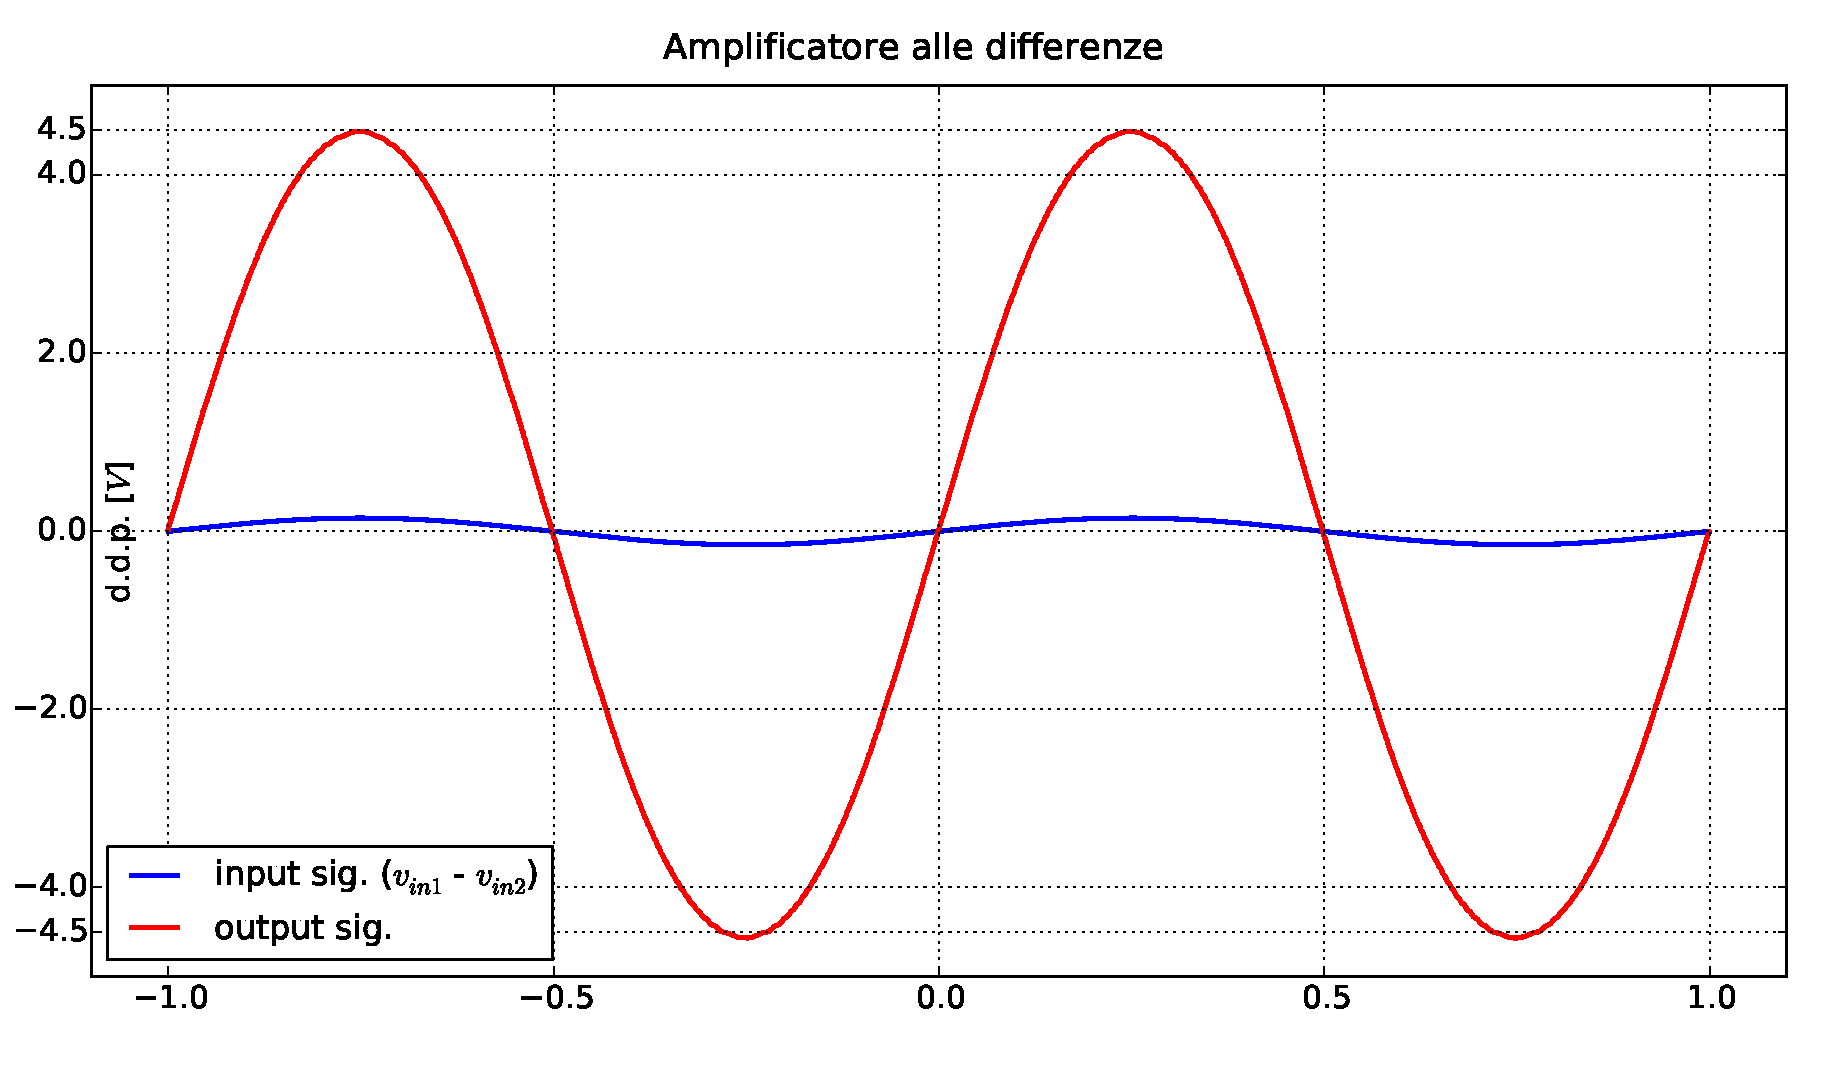
\includegraphics[scale=0.40025]{accontentati.pdf}
	\caption{Il segnale in blu è la differenza tra i segnali in entrata $v_{in1} - v_{in2}$. Nel nostro caso, avendo posto $v_{in2} = 0$, risulta verificato $v_{in1} - v_{in2} \,=\, v_{in1} \,=\, v_{in}$. Il segnale in rosso è il segnale in uscita al circuito $v_{out}$.}
	\label{fig:sig}
\end{figure}

\noindent Per rendere l'analisi dei segnali più semplice, abbiamo collegato $v_{in2}$ a terra.
Così facendo l'effetto dell'amplificatore alle differenze è stato quello di ottenere solo l'amplificazione del segnale in ingresso $v_{in1}$. 

Il valore sperimentale per il guadagno differenziale è stato stimato dai valori picco-picco del segnale in ingresso e di quello in output:

	$$G_{diff,exp}=\frac{V_{out,pp}}{V_{in,pp}} \, = \, 30.1 \pm 0.1$$

Invertendo eq. (\ref{eq:2}) e sfruttando la composozione degli errori è possibile calcolare il valore di resistenza intrinseca dell'emettitore:

$$ r_e \, = \, \frac{R_c}{2G_{diff}}-R_E \, = \, (46.7\pm0.8) \, \si{\ohm}$$

\noindent Per l'analisi del guadagno in modo comune, abbiamo collegato sia $v_{in1}$ che $v_{in2}$ al generatore di forme d'onda, in modo tale che entrambi i contatti fossero sempre allo stesso potenziale.
Ne abbiamo dunque calcolato il valore sperimentale confrontando i valori di tensione picco-picco e abbiamo ottenuto il modulo del guadagno in modo comune:

$$	G_{CM,exp} \,=\, -\frac{V_{out,pp}}{V_{in1,pp}} \, = \, -\frac{V_{out,pp}}{V_{in2,pp}} \, = \, -0.483 \pm 0.003$$

\noindent Ricordiamo che il guadagno in modo comune è definito negativo ed il segno meno indica solamente uno sfasamento tra i segnali di $\pi$.

Anche in questo caso abbiamo provato a calcolare il valore di $r_e$ partendo da eq. (\ref{eq:3}).

\begin{equation}
	r_e \, = \, -\frac{R_C+G_{CM}R_E+2G_{CM}R_1}{G_{CM}}
\end{equation}

\noindent In questo caso, tuttavia, piccole variazione di $G_{CM}$ producono una grande variazione per cui non risulta possibile stimare in modo preciso il valore di resistenza intrinseca dell'emettitore $r_e$ partendo da tale equazione.

Infine abbiamo calcolato il fattore di reiezione a modo comune (Common Mode Rejection Ratio):

\begin{equation}
CMRR=\frac{G_{diff}}{G_{CM}}=62.3\pm0.5
\end{equation}

Più tale fattore risulta alto e più l'amplificatore alle differenze è efficace.
Se ad esempio abbiamo un rumore identico su entrambi i canali di ingresso, un CMRR alto garantisce una riduzione di tale rumore sul segnale in output.

\section{Amplificatore alle differenze con sorgente di corrente}

Per migliorare il valore di $G_{CM}$ e di conseguenza quello di $CMRR$, si posiziona una sorgente di corrente costante a valle del circuito, come mostrato in Fig. \ref{fig:cc2}.
In questa seconda parte dell'esperienza ne abbiamo analizzato il comportamento.

\begin{wrapfigure}[19]{r}[0pt]{55mm}
	\caption{Schema dell'amplificatore alle differenze con sorgente di corrente costante.}
	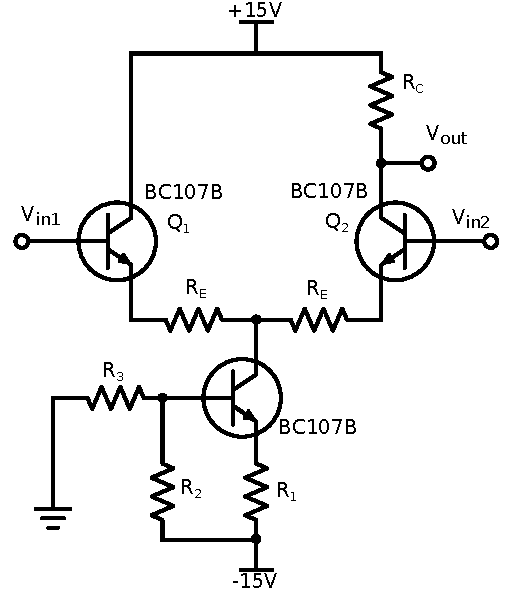
\includegraphics[width=55mm]{cc2.pdf}
	\label{fig:cc2}
\end{wrapfigure}

Abbiamo deciso di dimensionare le resistenze imponendo una corrente di collettore di \SI{1.5}{\milli\ampere} (così da avere una corrente di quiescenza di circa \SI{0.75}{\milli\ampere} attraverso ciascun transistor dell'amplificatore alle differenze) e una $R_1=1.5\si{\kilo\ohm}$ ( $R_1=(1.507 \pm 0.002)\si{\kilo\ohm}$). Possiamo dunque usare le relazioni $I_E=I_C+E_B \rightarrow I_E \approx I_C$, $I_E=\frac{V_E}{R_1}$ e $V_B=V_E+\SI{0.6}{\volt}$ per calcolare il valore di tensione di base necessario per ottenere una corrente di collettore di \SI{1.5}{\milli\ampere}. Successivamente, risulta immediato dimensionare le resistenze del partitore: 
\begin{equation}
V_B=(\frac{R_2}{R_2+R_3}-1) \cdot 15
\label{eq:casagay}
\end{equation}


In questo caso non possono essere determinate univocamente $R_2$ ed $R_3$ da eq. (\ref{eq:casagay}). È dunque nostro compito scegliere dei valori adeguati in modo da lasciar scorrere abbastanza corrente attraverso la base ma allo stesso tempo non dissipare troppa potenza sulle resistenze. Scegliendo un valore di $R_2=\SI{10}{\kilo\ohm}$ ($R_2=(9.933\pm0.002)\,\si{\kilo\ohm}$) otteniamo $R_3 \approx \SI{42.6}{\kilo\ohm}$. Nell'esperienza abbiamo utilizzato il valore suggerito dagli esercitatori di $\SI{33}{\kilo\ohm}$ ($(32.733 \pm 0.003)\,\si{\kilo\ohm}$). %#casalinoloprendeinculo 8=====D (*)

Il vantaggio di utilizzare una sorgente di corrente costante al posto della resistenza $R_1$ di Fig. \ref{fig:cc1} è quello di far scorrere sempre la stessa corrente nel circuito, indipendentemente dai segnali $v_{in1}$ e $v_{in2}$.
Ricordando la relazione $v_{out}=i_C R_C \simeq i_E R_C$, osserviamo che il segnale in uscita è direttamente proporzionale a $i_E$.
La sorgente di corrente, però, impone $I_E + i_E \simeq I_E$ e quindi, idealmente, il segnale in output sarà costante, cioè $v_{out}=0$.
In realtà, come già visto nella precedente esperienza, la sorgente di corrente costruita come mostrato in Fig. \ref{fig:cc2} non fornisce una corrente proprio costante.
Nonostante ciò, il $G_{CM}$ sarà molto piccolo e permetterà di ottenere un fattore di reiezione a modo comune molto grande.
%Al circuito sono state aggiunte due resistenze di valore $R_2 = (1507.5 \pm 0.5)\,\si{\ohm}$ e $R_3 = (32.723 \pm 0.003)\,\si{\kilo\ohm}$ e un ulteriore transistor BC107B.

\begin{wrapfigure}[19]{r}[0pt]{95mm}
	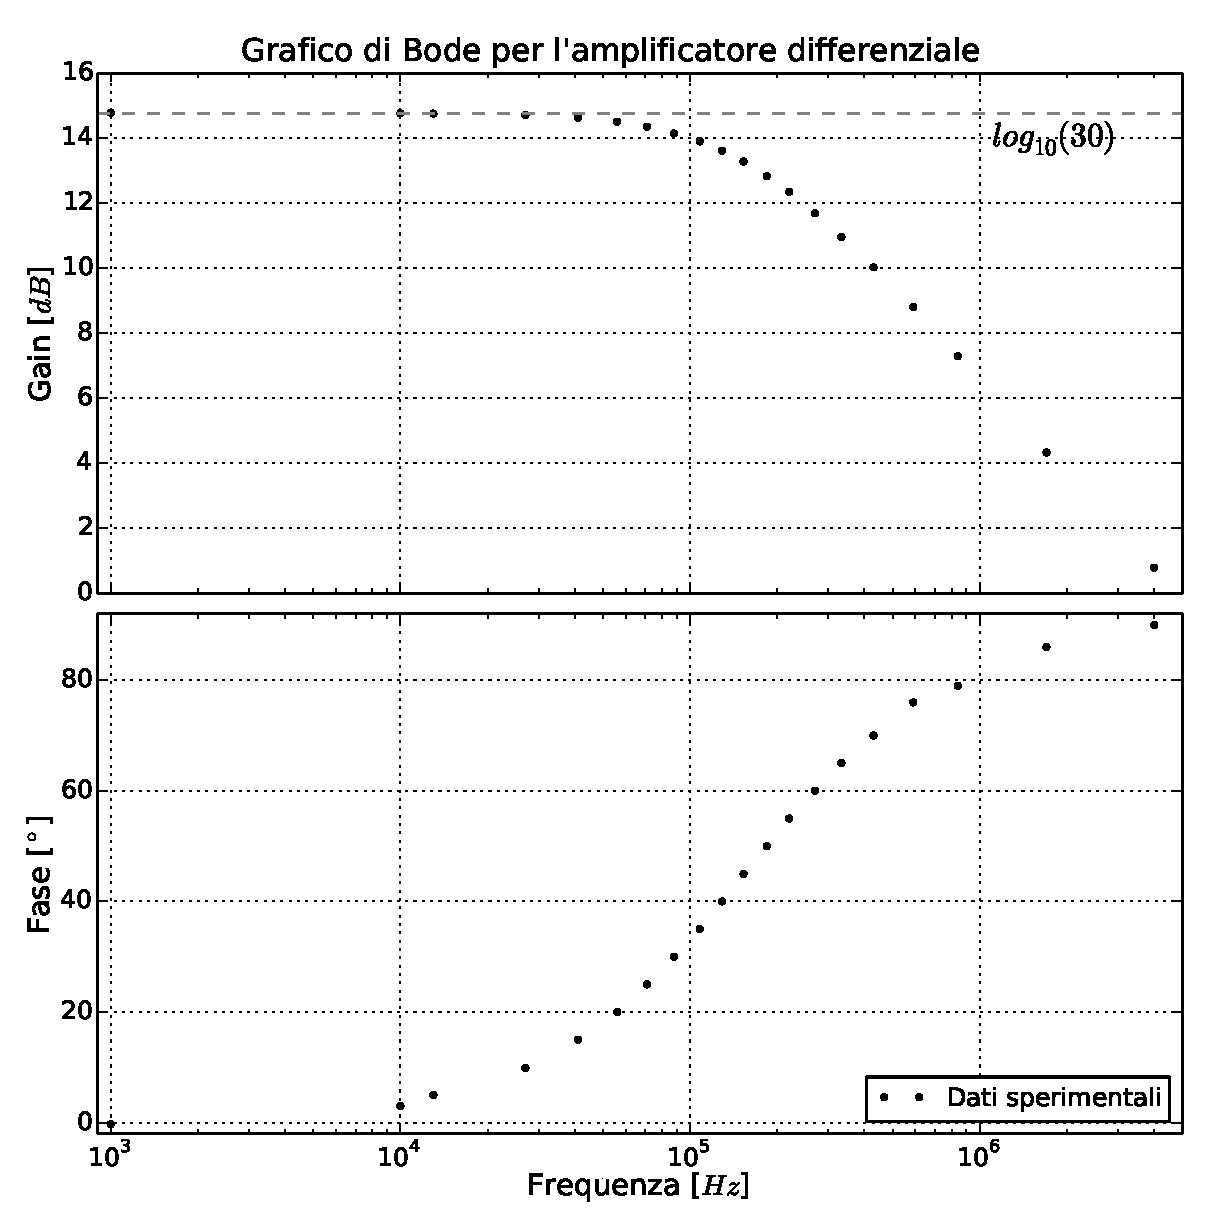
\includegraphics[width=95mm]{g1.pdf}
	\caption{Diagramma di Bode per l'amplificatore alle differenze. Il comportamento è simile a quello di un filtro passa basso.}
	\label{fig:bode}
\end{wrapfigure}

Abbiamo ricavato i valori del guadagno differenziale, del guadagno in modo comune e del fattore di reiezione a modo comune con relativi errori.

\noindent
\begin{minipage}{1\linewidth}
\begin{equation}
	G_{diff} = \frac{V_{out,pp}}{V_{in1,pp}} \, = \, 32.5 \,\pm\, 0.1
\end{equation}
\begin{equation}
	G_{CM} = -\frac{V_{out,pp}}{V_{in1,pp}} \, = \, -\frac{V_{out,pp}}{V_{in2,pp}} = -(7 \pm 1) \times 10^{-4}
\end{equation}
\begin{equation}
	CMRR = \frac{G_{diff}}{G_{CM}} = (50 \pm 7) \times 10^3
\end{equation}	
\end{minipage}%
%\begin{minipage}{.1\linewidth}
%\end{minipage}

Come vediamo il fattore di reiezione a modo comune è molto più grande (circa 3 ordini di grandezza) rispetto a quello ottenuto nella sezione precedente. 
